\chapter{Introduction}
\label{sec:intro}

\section{Hardware Non-Volatile Memory}


\textbf{Thesis Statement}: Malware on Mobile Operating Systems, especially Android, is better understood when not just analyzing the capabilities of an application, but the expectations the user has as to how it utilizes those capabilities as well.\\


\begin{smitemize}
\item Something1
\item Something2
\item Something3
\end{smitemize}


\begin{algorithm}[t]
\dontprintsemicolon
\linesnumbered

\SetAlFnt{\sf}
\SetAlCapFnt{\sf}

\SetKwFunction{GetLastConsistentVersion}{get\_last\_consistent\_version}
\SetKwFunction{GetNumEntries}{get\_num\_entries}
\SetKwFunction{NumLiveEntries}{num\_live\_entries}
\SetKwFunction{Insert}{insert}
\SetKwFunction{IsInnerNode}{is\_inner\_node}
\SetKwFunction{Lookup}{lookup}
\SetKwFunction{Find}{find}

\KwIn{k: key, r: root}
\KwOut{val: value}
\Begin(\Lookup{k, r}){
    $v \leftarrow  current\_version$\; \nllabel{line:l_version}
    $n \leftarrow r$\;
    \While { \IsInnerNode{n} } {  \nllabel{line:l_descend}
      $entry\_num \leftarrow \Find{k, n, v}$\; 
      $n \leftarrow n[entry\_num].child$\; \nllabel{line:l_descend_done}
    }
    $entry\_num \leftarrow \Find{k, n, v}$\; 
    \Return{$n[entry\_num].value$}\;
}
\BlankLine
\Begin(\Find{k, n, v}) {
  $l \leftarrow 0$\;
  $h \leftarrow \GetNumEntries{n}$\;
  \While(\tcp*[f]{Binary Serch}) { $l < h$ } { \nllabel{line:l_binary}
    $m \leftarrow (l + h)/2$\;
    \If { $k \leq n[m].key$ } {
      $h \leftarrow m-1$\;
    } \lElse $l \leftarrow m+1$\;   \nllabel{line:l_binary_done}
  }
  \While { $h < \GetNumEntries {n}$ } { \nllabel{line:vcheck}
    \If { $n[h].start \leq v$ } {
      \If { $n[h].end > v \quad \| \quad n[h].end = 0$ } {
        $break$\;
      }
    }
    $h \leftarrow h+1$\;  \nllabel{line:vcheck_done}
  }
  \Return{$h$}\;
}
\caption{CDDS B-Tree Lookup}
\label{alg:btree_lookup}
\end{algorithm}



\begin{table*}[t]
\begin{small}
\begin{center}
\begin{tabular}{c|cccccc}
Technology & Density  & \multicolumn{2}{c}{Read/Write Latency} & \multicolumn{2}{c}{Read/Write Energy} & Endurance \\
           & $\mu$m$^2$/bit & \multicolumn{2}{c}{ns}                 & \multicolumn{2}{c}{pJ/bit}  & writes/bit\\
\hline
HDD & 0.00006 & 3,000,000 & 3,000,000 & 2,500 & 2,500 & $\infty$ \\
Flash SSD (SLC) & 0.00210 & 25,000 & 200,000 & 250 & 250 & $10^5$ \\
DRAM (DIMM) & 0.00380  & 55 & 55 & 24 & 24 & $10^{18}$ \\
PCM & 0.00580 & 48 & 150 & 2 & 20 & $10^8$ \\
Memristor & 0.00580  & 100 & 100 & 2 & 2 & $10^8$
\end{tabular}
\end{center}
\end{small}
%\vspace{-0.2in}
\caption{Non-Volatile Memory Characteristics: 2015 Projections}
\label{tab:nvbm}
%\vspace{-0.1in}
\end{table*}

\begin{figure}[t]
\begin{center}
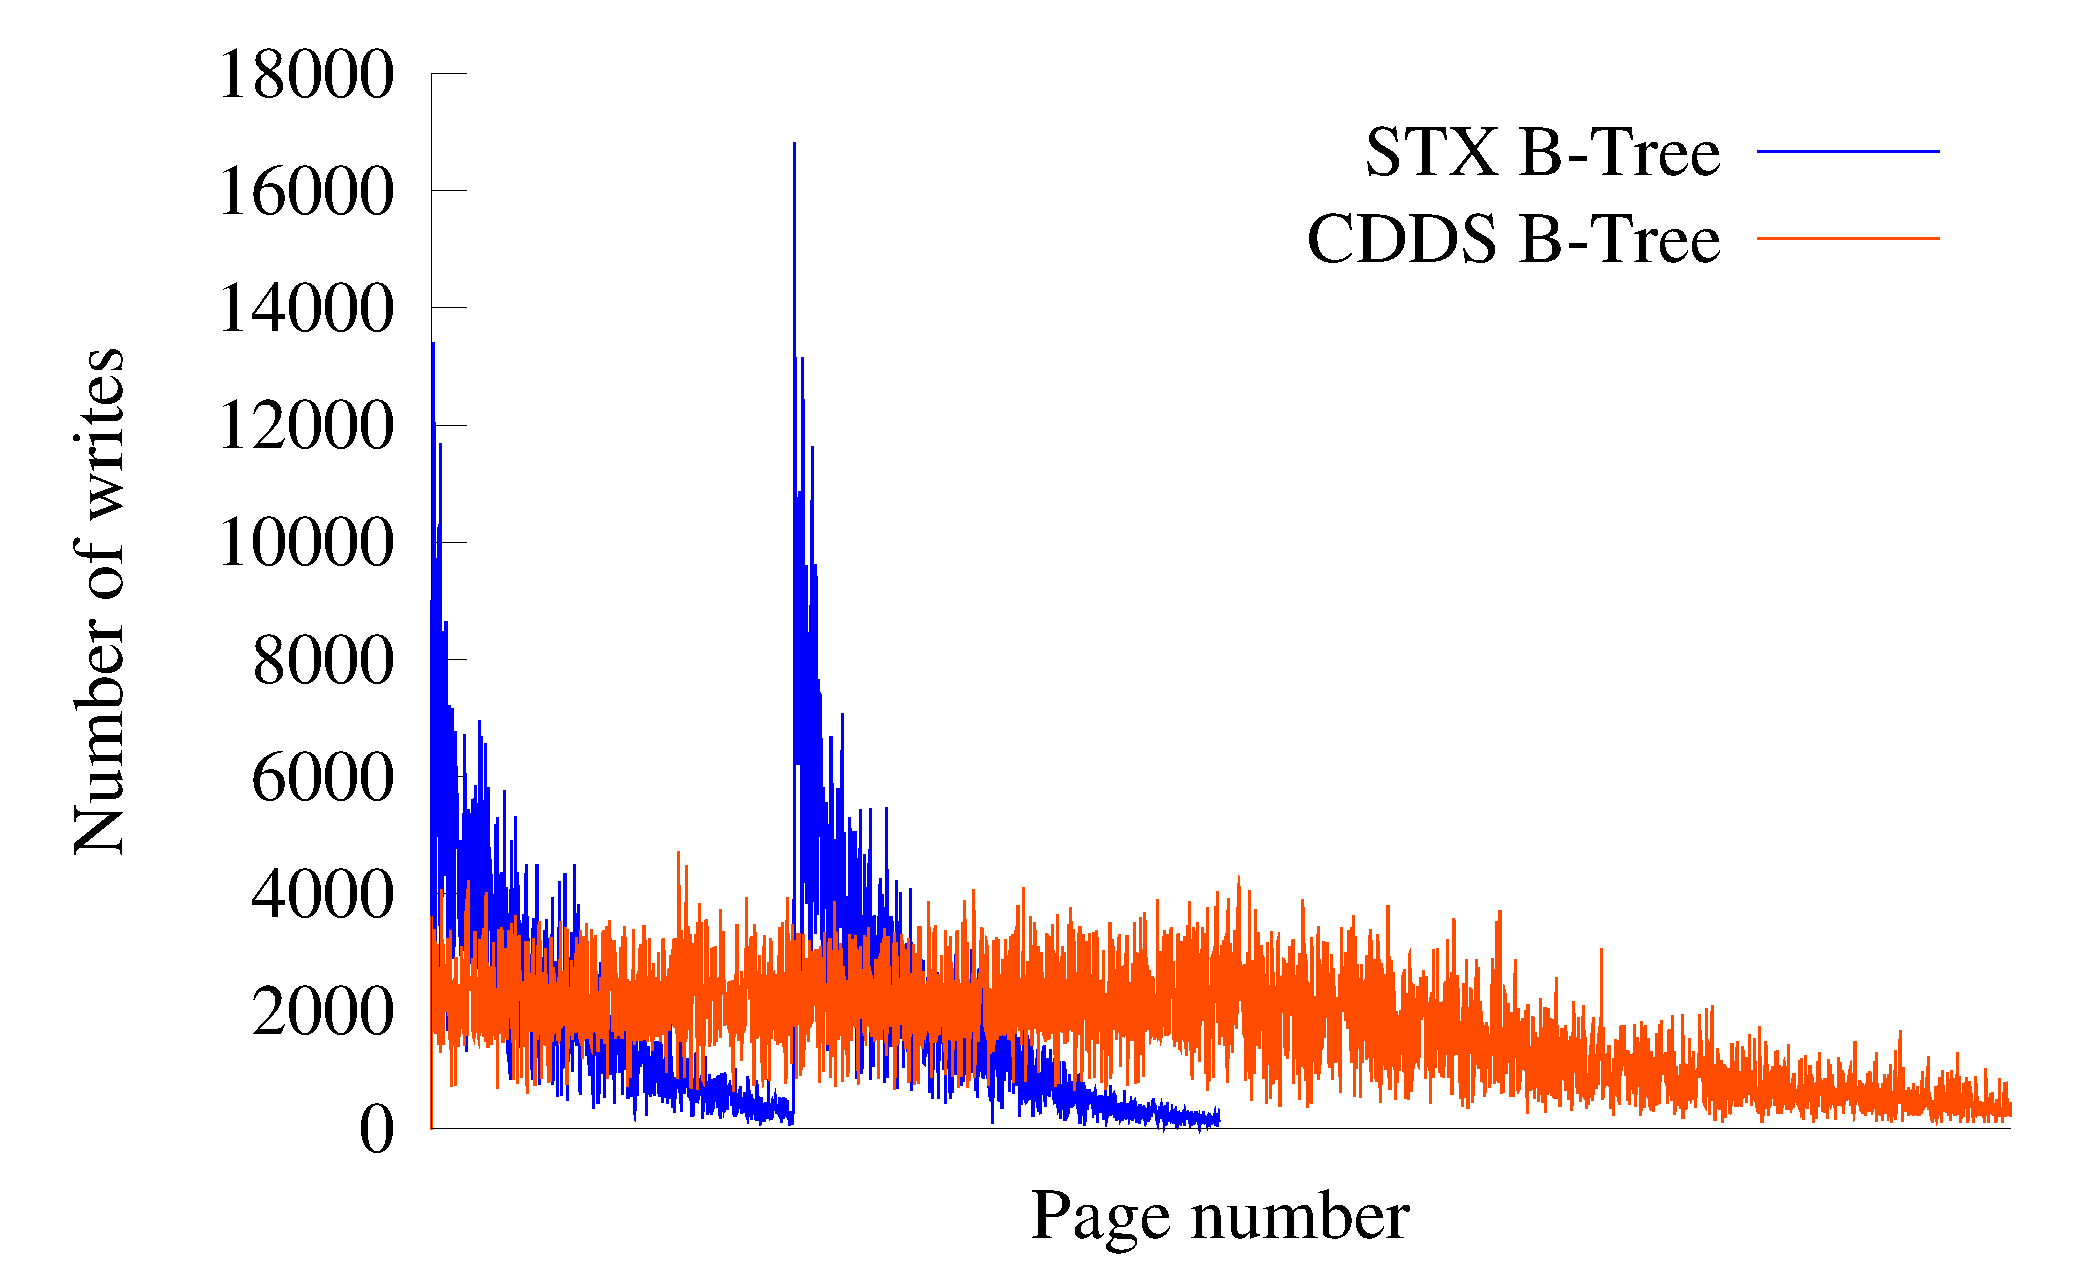
\includegraphics[width=0.7\columnwidth]{figs/wear-line}
\caption{Number of writes per page in CDDS B-Tree and STX B-Tree}
\label{fig:wear-line}
\end{center}
\end{figure}



\section{Flush Performance}
\label{sec:flush_perf}

\begin{figure}[t]
\begin{minipage}[b]{0.49\linewidth}
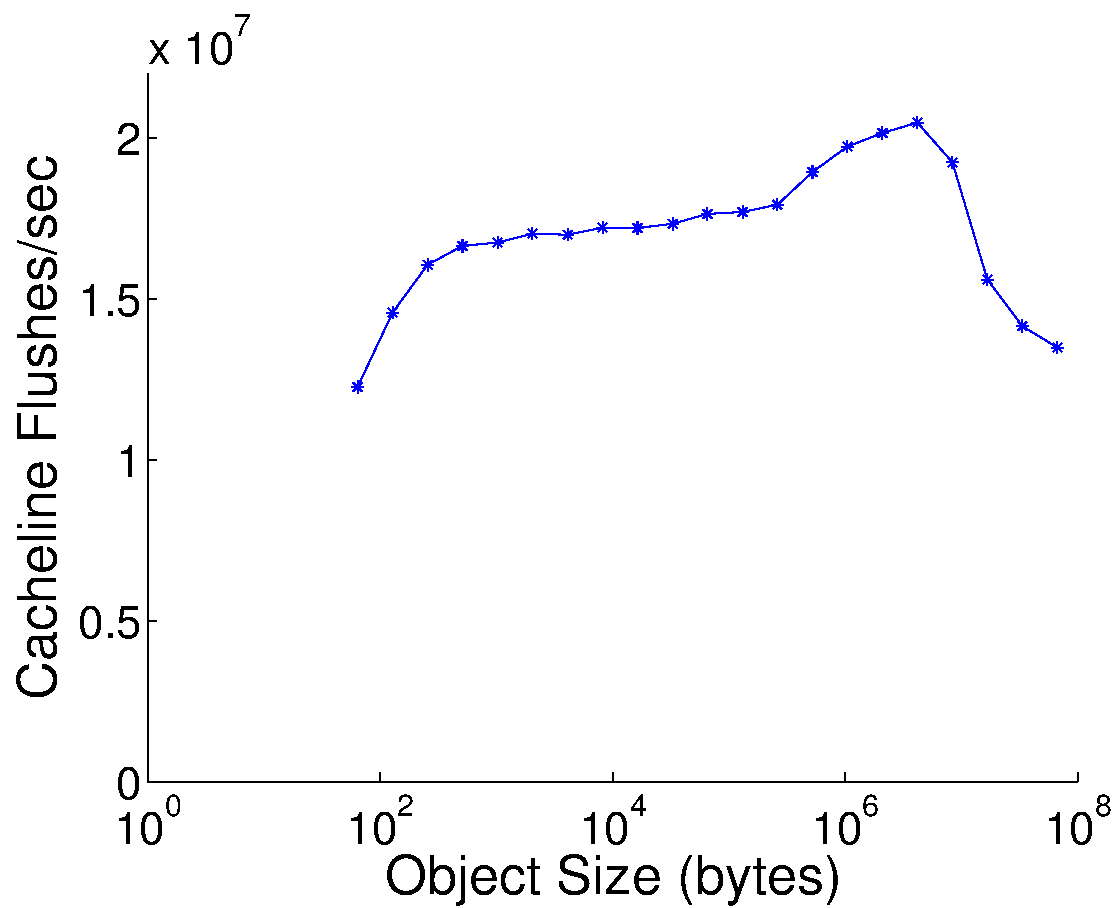
\includegraphics[width=\columnwidth]{figs/flushes_per_sec}
%\vspace{-0.3in}
\caption{Flushes/second}
\label{fig:flushes_per_sec}
\end{minipage}
%\hspace{0.1cm}
\begin{minipage}[b]{0.49\linewidth}
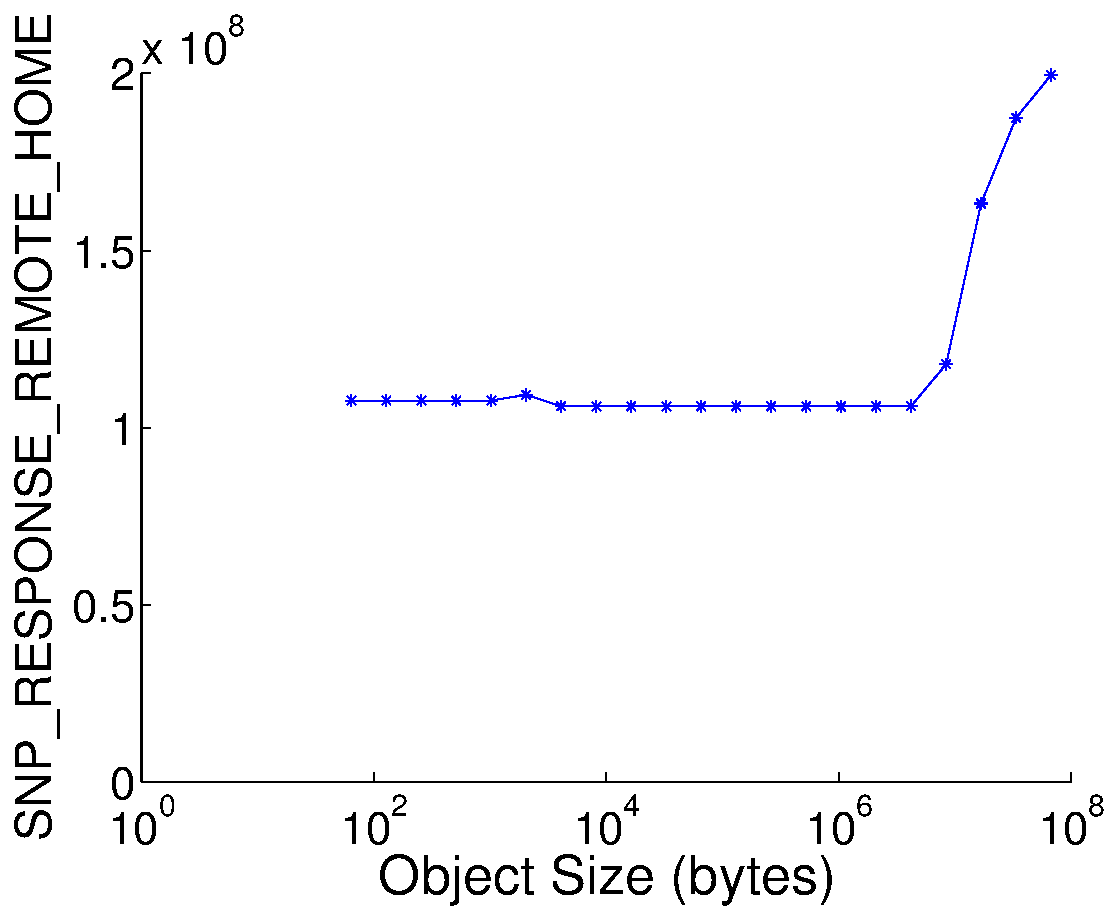
\includegraphics[width=\columnwidth]{figs/snoop_response}
%\vspace{-0.3in}
\caption{Cache Snooping}
\label{fig:ext_snoop}
\end{minipage}
%\vspace{-0.15in}
\end{figure}




% XXX - Say something about bandwidth below?

Table~\ref{tab:nvbm} summarizes key attributes of potential storage
Chapter~\ref{sec:flush_perf} 
40nm~\citep{ITRS07,Mandelman02,Mueller05}.  Additionally, power


\textit{file interface}
\textbf{Thesis Statement}:
\\
\texttt{flush}


\begin{sloppypar}
SUPER_VERY_LONG_WORDS_APPARENTLY_NEED_THIS
\end{sloppypar}


Tembo\footnote{Swahili for elephant, an animal anecdotally known forits memory.}, our Key-Value (KV) store described in


Memristors can be used to provide a single ``unified data-store''







replace all ’ with '

